\documentclass{beamer}

\usetheme{Berkeley}
\usepackage{graphicx}
\graphicspath{ {./images/} }

\title{Final Delivery Presentation}

\subtitle{IO and Algorithm}

\author{Albert van Kiel, Timo Hermsen, Robin Baneke, Max van Hasselt, Robert Kleef and Menno Prinzhorn}

\date{\today}

\begin{document}

\begin{frame}
    \titlepage
\end{frame}

\section{Background}
    
\begin{frame}{Background}
    Project background
    \\~\\
    \begin{itemize}
        \item SIGPROC library
        \item eScience center
        \item Asteria
        \item IO/Algorithm
    \end{itemize}
\end{frame}

\section{Goals}
\begin{frame}{Goals}
    Our goals for Asteria      
	\begin{itemize}
		\item Refactoring SIGPROC library
		\item Open Source and well documented for the world to use
		\begin{itemize}
			\item GNU Lesser General Public License v3.0
		\end{itemize}
		\item Ability to be maintained and improved by future students
        \item Python/C++
        \begin{itemize}
			\item Python for the initial software.
			\item C++ Later for possible improved performance and/or GPU Support
		\end{itemize}
        \item Tests require a mimimum of 60\% of code coverage
    \end{itemize}
\end{frame}

\section{Methodology}
	\begin{frame}{Methodology}
	How we ensured proper team-work processes
	\begin{itemize}
		\item Agile Development (SCRUM)
		\item Sprint plannings, reviews and retrospectives
		\item Issue tracking by Trello
		\item Pull requests and mergers
	\end{itemize}
\end{frame}

\section{Quality Assurance and CI/CD}
\begin{frame}{Quality Assurance and (CI)/CD}
    Quality Assurance and Automated building    
	\begin{itemize}
		\item Ran by Travis
		\item Linting PyLint to ensure coding standards
		\item PyTest to maintain greater than 60 percent code coverage
		\item 90 Percent code coverage reached
		\item Manual QA using Pull requests
    \end{itemize}
\end{frame}

\section{Module based design}
\begin{frame}{Module based Design}
	\begin{itemize}
		\item Based on a lot of Python libraries such as matplotlib. 
		\item Ensures that each seperate module can be used seperatly in different types of Python software. 
		\item For example: The filterbank module can be used seperatly from the timeseries module. 
	\end{itemize}
\end{frame}


\section{Modules}
\begin{frame}{Modules}
	These modules are present and usable in the Asteria library     
	\begin{itemize}
		\item Filterbank
		\item Clipping
		\item Dedisperse
		\item Timeseries
		\item Fourier
		\item Pipeline
		\item Plot
	\end{itemize}
\end{frame}

\section{Filterbank}
\begin{frame}{Filterbank}
	\begin{itemize}
		\item Generate mock data
		\begin{itemize}
			\item Generate header
			\item Generate signal which does include a Pulsar
			\item Exports to filterbank file
		\end{itemize}
		\item Read filterbank files into special Filterbank object
	\end{itemize}
\end{frame}

\section{Clipping}
\begin{frame}{Clipping}
	\begin{columns}
		\begin{column}{0.5\textwidth}
			Filter samples with noise
			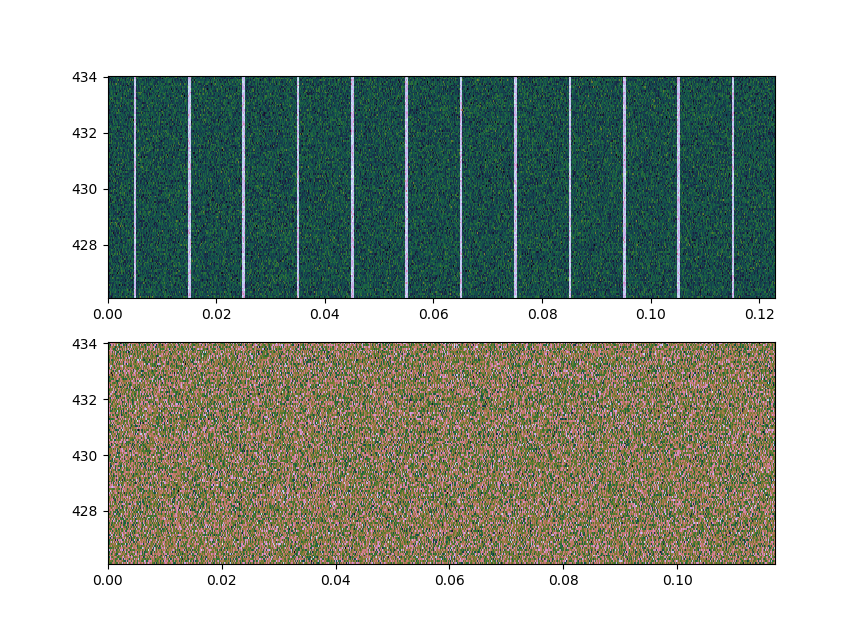
\includegraphics[width=\columnwidth]{filter_samples}
		\end{column}
		\begin{column}{0.5\textwidth}
			Filter frequencies with noise
			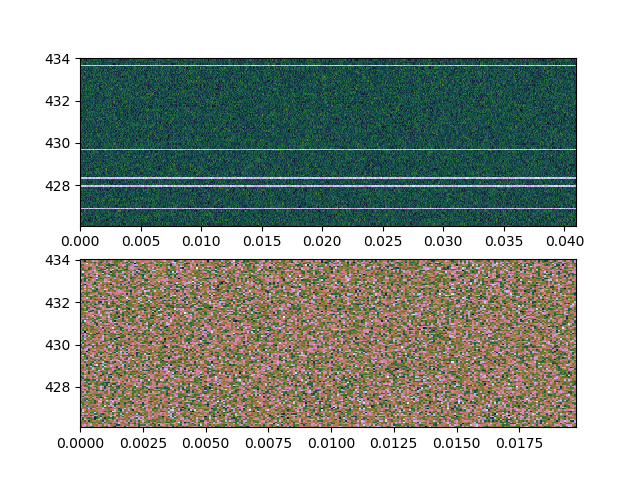
\includegraphics[width=\columnwidth]{filter_freqs}
		\end{column}
	\end{columns}
\end{frame}

\section{Dedisperse}
\begin{frame}{Dedisperse}
	Dedispersion
\end{frame}

\section{Timeseries}
\begin{frame}{Timeseries}
	\begin{itemize}
		\item Object is able to be initialized from 1D Array
		\item Object is able to be initialized from Filterbank
		\item Implemented downsampling
		\item All future timeseries operations shall be included here
	\end{itemize}
\end{frame}

\section{Fourier}
\begin{frame}{Fourier}
	\begin{itemize}
		\item FFT Matrix
		\item Discrete Fourier Transform
		\item Cooley-Tukey
		\item Shirt zero-frequency
	\end{itemize}
\end{frame}

\section{Pipeline}
\begin{frame}{Pipeline}
	\begin{figure}
		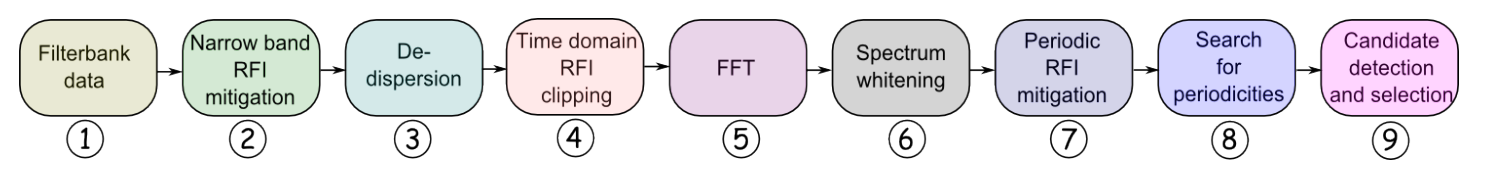
\includegraphics[width=\textwidth]{pipeline-order}
	\end{figure}
\end{frame}

\section{Plot}
\begin{frame}{Plot}
	\begin{itemize}
		\item Plot
		\item Waterfall
	\end{itemize}
\end{frame}

\section{Results and Benchmarks}
\begin{frame}{Results and Benchmarks}
	\begin{itemize}
		\item Ran on Centos 6, 32GB RAM, Dual Xeon Quad Core (HvA Server)
	\end{itemize}
\end{frame}

\section{Run time 3070 Samples in seconds}
\begin{frame}{Run time 3070 Samples in seconds}
	\begin{figure}
		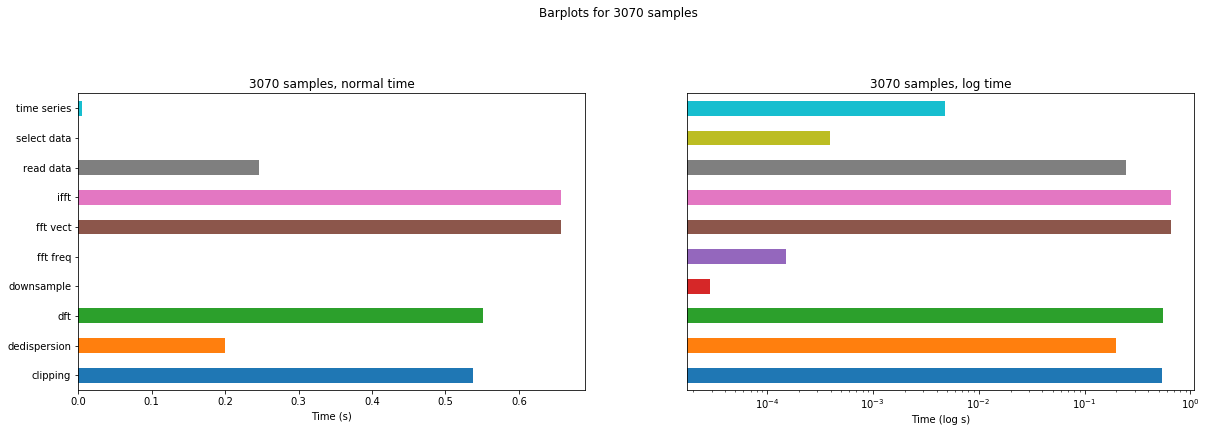
\includegraphics[width=\textwidth]{barchart_3070}
	\end{figure}
\end{frame}

\section{Run time 49150 Samples in seconds}
\begin{frame}{Run time 49150 Samples in seconds}
	\begin{figure}
		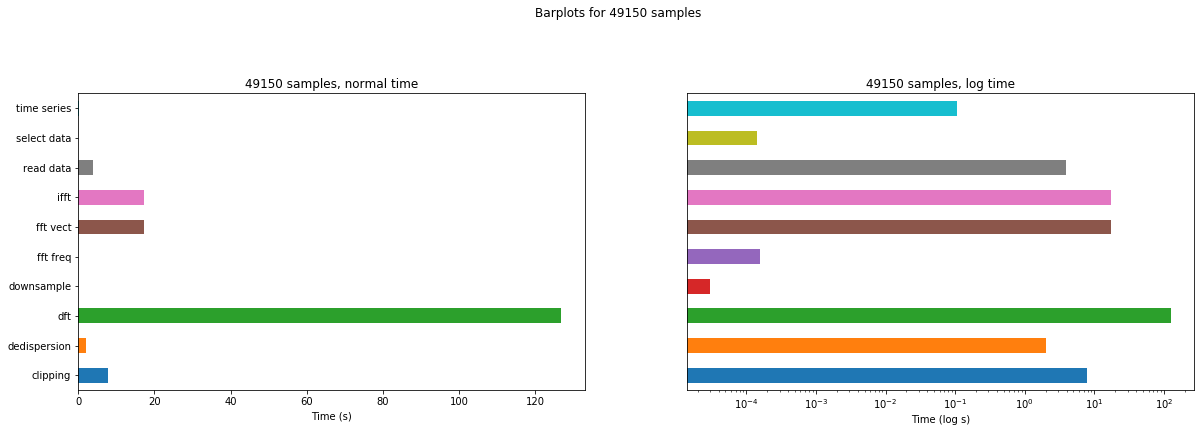
\includegraphics[width=\textwidth]{barchart_49150}
	\end{figure}
\end{frame}

\section{Distribution of time 49150 Samples}
\begin{frame}{Distribution of time 49150 Samples}
	\begin{figure}
		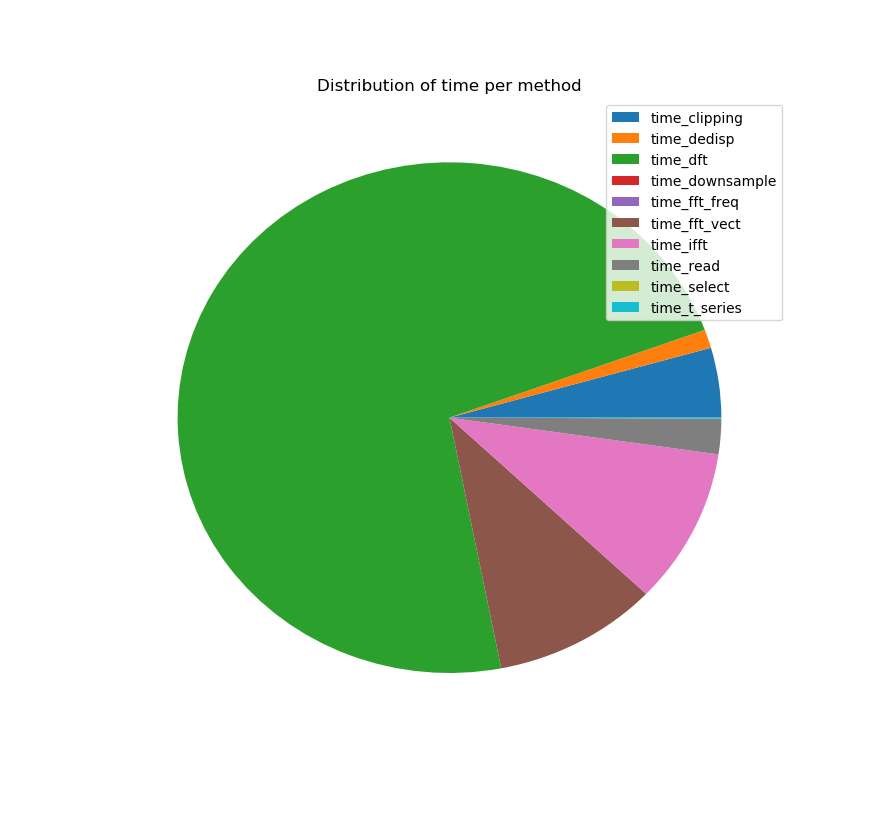
\includegraphics[width=.8\textwidth]{piechart_49150}
	\end{figure}
\end{frame}


\section{End}
\begin{frame}{Questions?}
	Questions?
\end{frame}

\end{document}
